\documentclass{article}
\usepackage[margin=0.7in]{geometry}
\usepackage{graphicx}
\usepackage{booktabs}
\usepackage{caption}
\usepackage{float}
\usepackage{subcaption}

\title{Demand Estimation Report}
\author{Airlines Merger Simulation}
\date{\today}

\begin{document}

\maketitle

\section{Introduction}
This report presents the results of the demand estimation analysis conducted as part of the Airlines Merger Simulation project. The tables and figures included here summarize the key findings.

The model specification follows a logit and nested-logit framework, where consumer utility is modeled as:
\begin{itemize}
    \item \textbf{Logit Model:} $\ln(s_{jt}) - \ln(s_{0t}) = \alpha p_{jt} + x_{jt} \beta + \xi_t + \xi_{jt} + \epsilon_{ijt}$
    \item \textbf{Nested-Logit Model:} $\ln(s_{jt}) - \ln(s_{0t}) = \alpha p_{jt} + x_{jt} \beta + \sigma \ln(s_{jt|g}) + \xi_t + \xi_{jt} + \epsilon_{ijt}$
\end{itemize}
where:
\begin{itemize}
    \item $p_{jt}$ is the average fare (price).
    \item $x_{jt}$ includes regressors such as share nonstop, average distance, squared distance, and log(1 + number of fringe carriers).
    \item $\nu_t$ and $\xi_{jt}$ are fixed effects for origin-destination and product-level unobservables.
    \item $s_{jt|g}$ is the share of product $j$ in group $g$.
    \item $\sigma$ captures the nesting parameter in the nested-logit model.
    \item Instruments ($z^D_{jt}$) include average rival presence, average number of markets served by rivals, and the number of rival carriers.
\end{itemize}


\section{Summary Statistics}


\begin{table}[htbp]\centering
\def\sym#1{\ifmmode^{#1}\else\(^{#1}\)\fi}
\caption{Summary statistics: variables used in demand estimation}
\begin{tabular}{l*{1}{ccccccc}}
\toprule
                    &\multicolumn{7}{c}{}                                                                      \\
                    &        mean&          sd&         min&         p25&         p50&         p75&         max\\
\midrule
Market share        &       0.001&       0.006&      0.0000&      0.0001&       0.000&       0.001&       0.473\\
Outside share       &       0.992&       0.016&      0.3365&      0.9910&       0.996&       0.998&       1.000\\
Inside share sum    &       0.008&       0.016&      0.0002&      0.0024&       0.004&       0.009&       0.664\\
Nest share          &       0.008&       0.016&      0.0002&      0.0024&       0.004&       0.009&       0.664\\
Number of rival carriers&       5.477&       2.274&      1.0000&      4.0000&       5.000&       7.000&      22.000\\
Number of destinations served&      51.458&      31.554&      1.0000&     27.0000&      47.000&      75.000&     137.000\\
Average fare (dollars)&     226.831&      93.858&     25.0000&    172.4141&     212.830&     260.995&    2489.196\\
Share nonstop flights &       0.195&       0.355&      0.0000&      0.0000&       0.000&       0.143&       1.000\\
Average Distance (000s miles)&       1.491&       0.856&      0.0670&      0.8752&       1.298&       1.995&      10.345\\
Average Distance sqr (000s miles)&       2.958&       3.700&      0.0045&      0.7659&       1.686&       3.980&     107.019\\
Log(1 + fringe carriers)&       0.408&       0.469&      0.0000&      0.0000&       0.000&       0.693&       2.565\\
\midrule
Observations        &     1371742&            &            &            &            &            &            \\
\bottomrule
\end{tabular}
\end{table}


\pagebreak
\section{Demand Estimation Results}

Column (1) presents the results of the logit model without instruments,
while column (2) shows the logit model results with price instruments. 
Column (3) shows the nested-logit model without instruments, and 
column (4) presents the nested-logit model with instruments for both prices and nest shares.  The nests are defined as inside goods (carriers that are not the outside good) and outside good.
All columns include fixed effects for origin-destination markets. Robust standard errors are reported in parentheses below the coefficients.


%The coefficients are interpreted as elasticities, with standard errors clustered at the market level.
\begin{table}[htbp]\centering
\def\sym#1{\ifmmode^{#1}\else\(^{#1}\)\fi}
\caption{Demand Estimates (Logit and Nested-Logit)}
\begin{tabular}{l*{4}{c}}
\toprule
                    &\multicolumn{1}{c}{(1)}&\multicolumn{1}{c}{(2)}&\multicolumn{1}{c}{(3)}&\multicolumn{1}{c}{(4)}\\
                    &\multicolumn{1}{c}{ln(s\_jt) - ln(s\_0t)}&\multicolumn{1}{c}{ln(s\_jt) - ln(s\_0t)}&\multicolumn{1}{c}{ln(s\_jt) - ln(s\_0t)}&\multicolumn{1}{c}{ln(s\_jt) - ln(s\_0t)}\\
\midrule
Average ticket price&     -0.0024\sym{***}&      0.0318\sym{***}&     -0.0004\sym{***}&     -0.0019\sym{***}\\
                    &    (0.0000)         &    (0.0004)         &    (0.0000)         &    (0.0001)         \\
\addlinespace
Share nonstop flights &      1.9793\sym{***}&      1.8355\sym{***}&      0.0946\sym{***}&      0.3154\sym{***}\\
                    &    (0.0053)         &    (0.0130)         &    (0.0009)         &    (0.0043)         \\
\addlinespace
Average Distance (000s miles)&     -4.1108\sym{***}&     -5.6862\sym{***}&     -0.0442\sym{***}&     -0.4475\sym{***}\\
                    &    (0.0159)         &    (0.0692)         &    (0.0024)         &    (0.0153)         \\
\addlinespace
Average Distance sqr (000s miles)&      0.2929\sym{***}&      0.1273\sym{***}&      0.0046\sym{***}&      0.0440\sym{***}\\
                    &    (0.0038)         &    (0.0174)         &    (0.0005)         &    (0.0014)         \\
\addlinespace
Log(1 + fringe carriers)&     -0.4908\sym{***}&     -0.1865\sym{***}&      0.0702\sym{***}&     -0.0056\sym{***}\\
                    &    (0.0037)         &    (0.0083)         &    (0.0006)         &    (0.0010)         \\
\addlinespace
ln(s\_jt) - ln(s\_gt) &                     &                     &      0.9809\sym{***}&      0.8688\sym{***}\\
                    &                     &                     &    (0.0002)         &    (0.0024)         \\
\midrule
Observations        &     1371742         &     1371742         &     1371742         &     1371742         \\
Adjusted \(R^{2}\)  &       0.486         &      -1.674         &       0.985         &       0.973         \\
F-statistic (IV)    &                     &   3738.9612         &                     &    422.5438         \\
\bottomrule
\end{tabular}
\end{table}


\section{Elasticities}
\centering

\begin{table}[htbp]\centering
\def\sym#1{\ifmmode^{#1}\else\(^{#1}\)\fi}
\caption{Elasticities: Own-price (Logit and Nested-Logit)}
\begin{tabular}{l*{1}{cccccccc}}
\toprule
                    &\multicolumn{8}{c}{}                                                                                   \\
                    &       count&        mean&          sd&         min&         p25&         p50&         p75&         max\\
\midrule
Logit Elasticity    &     1371742&      -0.548&       0.227&      -6.021&      -0.631&      -0.514&      -0.417&      -0.060\\
Nested-Logit Elasticity&     1371742&      -3.224&       1.353&     -34.953&      -3.750&      -3.038&      -2.422&      -0.092\\
\midrule
Observations        &     1371742&            &            &            &            &            &            &            \\
\bottomrule
\end{tabular}
\end{table}


\begin{figure}[htbp]
    \centering
    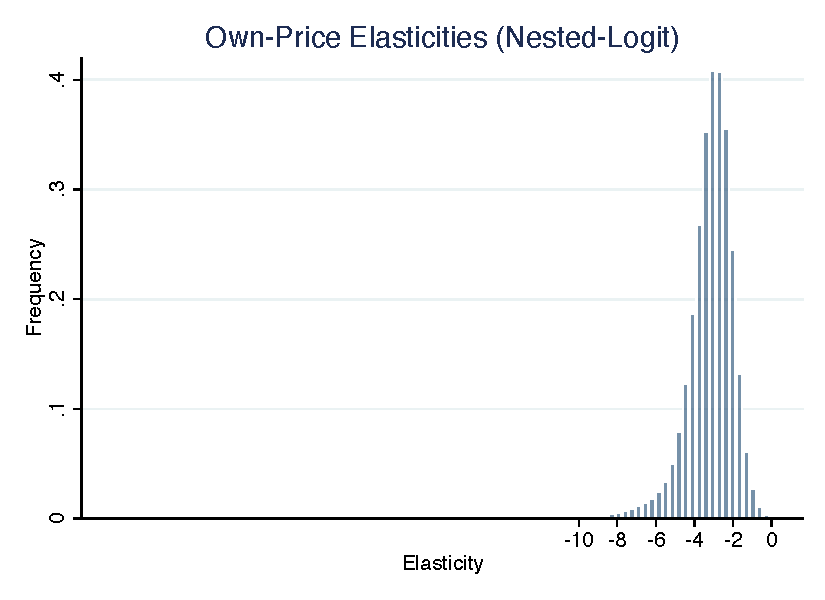
\includegraphics[width=0.8\textwidth]{../src/output/elasticity_logit_histogram.pdf}
    \caption{Histogram of Elasticities}
\end{figure}

\pagebreak
\section{Appendix: First Stage Results}
{
\def\sym#1{\ifmmode^{#1}\else\(^{#1}\)\fi}
\begin{tabular}{l*{1}{c}}
\toprule
                    &\multicolumn{1}{c}{(1)}\\
                    &\multicolumn{1}{c}{Average fare (dollars)}\\
\midrule
Average distance to rival markets&      0.0359\sym{***}\\
                    &    (0.0008)         \\
\addlinespace
Average number of rival destinations&     -0.8452\sym{***}\\
                    &    (0.0088)         \\
\addlinespace
Number of rival carriers&    -10.9626\sym{***}\\
                    &    (0.0668)         \\
\addlinespace
Number of rival carriers lower nest&      7.8044\sym{***}\\
                    &    (0.0433)         \\
\addlinespace
Share nonstop flights &     -1.9907\sym{***}\\
                    &    (0.3057)         \\
\addlinespace
Average Distance (000s miles)&     44.5059\sym{***}\\
                    &    (1.8443)         \\
\addlinespace
Average Distance sqr (000s miles)&      4.5607\sym{***}\\
                    &    (0.4781)         \\
\addlinespace
Log(1 + fringe carriers)&      3.0140\sym{***}\\
                    &    (0.2175)         \\
\midrule
Observations        &     1636916         \\
\bottomrule
\multicolumn{2}{l}{\footnotesize Standard errors in parentheses}\\
\multicolumn{2}{l}{\footnotesize \sym{*} \(p<0.10\), \sym{**} \(p<0.05\), \sym{***} \(p<0.01\)}\\
\end{tabular}
}


{
\def\sym#1{\ifmmode^{#1}\else\(^{#1}\)\fi}
\begin{tabular}{l*{1}{c}}
\toprule
                    &\multicolumn{1}{c}{(1)}\\
                    &\multicolumn{1}{c}{ln(s\_jt) - ln(s\_gt)}\\
\midrule
Average distance to rival markets&      0.0016\sym{***}\\
                    &    (0.0000)         \\
\addlinespace
Average number of rival destinations&     -0.0193\sym{***}\\
                    &    (0.0002)         \\
\addlinespace
Number of rival carriers&     -0.2889\sym{***}\\
                    &    (0.0011)         \\
\addlinespace
Share nonstop flights &      1.8861\sym{***}\\
                    &    (0.0045)         \\
\addlinespace
Average Distance (000s miles)&     -3.8357\sym{***}\\
                    &    (0.0122)         \\
\addlinespace
Average Distance sqr (000s miles)&      0.2393\sym{***}\\
                    &    (0.0027)         \\
\addlinespace
Log(1 + fringe carriers)&     -0.0480\sym{***}\\
                    &    (0.0038)         \\
\midrule
Observations        &     1636916         \\
\bottomrule
\multicolumn{2}{l}{\footnotesize Standard errors in parentheses}\\
\multicolumn{2}{l}{\footnotesize \sym{*} \(p<0.10\), \sym{**} \(p<0.05\), \sym{***} \(p<0.01\)}\\
\end{tabular}
}

\end{document}
